%%%%%%%%%%%%%%%%%%%%%%%%%%%%%%%%%%%%%%%%%
% Journal Article
% LaTeX Template
% Version 1.3 (9/9/13)
%
% This template has been downloaded from:
% http://www.LaTeXTemplates.com
%
% Original author:
% Frits Wenneker (http://www.howtotex.com)
%
% License:
% CC BY-NC-SA 3.0 (http://creativecommons.org/licenses/by-nc-sa/3.0/)
%
%%%%%%%%%%%%%%%%%%%%%%%%%%%%%%%%%%%%%%%%%

%----------------------------------------------------------------------------------------
%	PACKAGES AND OTHER DOCUMENT CONFIGURATIONS
%----------------------------------------------------------------------------------------

\documentclass[twoside]{article}

\usepackage{lipsum} % Package to generate dummy text throughout this template
\usepackage[french]{babel}

\usepackage[utf8]{inputenc}

\usepackage[sc]{mathpazo} % Use the Palatino font
\usepackage[T1]{fontenc} % Use 8-bit encoding that has 256 glyphs
\linespread{1.05} % Line spacing - Palatino needs more space between lines
\usepackage{microtype} % Slightly tweak font spacing for aesthetics

\usepackage[hmarginratio=1:1,top=32mm,columnsep=20pt]{geometry} % Document margins
\usepackage{multicol} % Used for the two-column layout of the document
\usepackage[hang, small,labelfont=bf,up,textfont=it,up]{caption} % Custom captions under/above floats in tables or figures
\usepackage{booktabs} % Horizontal rules in tables
\usepackage{float} % Required for tables and figures in the multi-column environment - they need to be placed in specific locations with the [H] (e.g. \begin{table}[H])
\usepackage{hyperref} % For hyperlinks in the PDF

\usepackage{lettrine} % The lettrine is the first enlarged letter at the beginning of the text
\usepackage{paralist} % Used for the compactitem environment which makes bullet points with less space between them
\usepackage{graphicx}

\usepackage{abstract} % Allows abstract customization
\renewcommand{\abstractnamefont}{\normalfont\bfseries}
\renewcommand{\abstractname}{Résumé} % Set the "Abstract" text to bold
\renewcommand{\abstracttextfont}{\normalfont\small\itshape} % Set the abstract itself to small italic text

\usepackage{titlesec} % Allows customization of titles
\renewcommand\thesection{\Roman{section}} % Roman numerals for the sections
\renewcommand\thesubsection{\arabic{subsection}.\arabic{subsection}} % Roman numerals for subsections
\titleformat{\section}[block]{\bfseries\large\scshape\centering}{\thesection.}{1em}{} % Change the look of the section titles
\titleformat{\subsection}[block]{\bfseries\large}{\thesubsection.}{1em}{} % Change the look of the section titles

\usepackage{fancyhdr} % Headers and footers
\pagestyle{fancy} % All pages have headers and footers
\fancyhead{} % Blank out the default header
\fancyfoot{} % Blank out the default footer
\renewcommand{\headrulewidth}{0pt} %pour enlever la ligne du header
%\fancyhead[C]{titre, date, noms...	} % Custom header text
\fancyfoot[RO,LE]{\thepage} % Custom footer text


%agrandissement de la zone de texte
\addtolength{\oddsidemargin}{-1cm}
\addtolength{\evensidemargin}{-1cm}
\addtolength{\textwidth}{2cm}

%pour les maths
\usepackage{amsmath}
\usepackage{amsfonts}
\usepackage{todonotes}
%----------------------------------------------------------------------------------------
%	TITLE SECTION
%----------------------------------------------------------------------------------------

\title{\vspace{-15mm}\fontsize{24pt}{10pt}\selectfont\textbf{Identification de défauts par onde de Lamb}} % Article title

\author{
\large
{Alice \textsc{Dinsenmeyer} \& Thomas \textsc{Lechat}}\\[2mm] % Your name %\thanks{}
%\normalsize University of California \\ % Your institution
%\normalsize \href{mailto:john@smith.com}{john@smith.com} % Your email address
\vspace{-5mm}
}
\date{}

%----------------------------------------------------------------------------------------

\begin{document}

\maketitle % Insert title

\thispagestyle{fancy} % All pages have headers and footers

%----------------------------------------------------------------------------------------
%	ABSTRACT
%----------------------------------------------------------------------------------------

\begin{abstract}
L'utilisation d'ondes guidées dans les plaques est présentée ici pour des applications de contrôle non-destructif. Les ondes de Lamb proviennent de la recombinaisons d'ondes longitudinales et transversales dans les plaques. Une première étude des modes de Lamb est faite sur une plaque d'aluminium: les résultats ne sont pas probants dès lors qu'on cherche à mettre en évidence d'autres modes que le plus basique (A0). Les trains d'ondes se propageant à des vitesses différentes sont trop difficiles à dissocier. Dans un second temps, un mobile industriel est utilisé pour contrôler un tuyau d'acier. Le mobile utilise un EMAT qu'il est possible de régler pour générer le mode voulu. Le dispositif permet de facilement retrouver les défauts présents sur le tuyau (qui sont visibles à l’œil nu).

\end{abstract}

%----------------------------------------------------------------------------------------
%	ARTICLE CONTENTS
%----------------------------------------------------------------------------------------

\begin{multicols}{2} % Two-column layout throughout the main article text

\section{Introduction}
Différents types d'ondes élastiques sont connus dans la propagation dans la matière. Ces ondes peuvent être séparées en 2 catégories: les ondes locales (longitudinales et transversales) qui sont solutions de l'équation d'onde en milieu infini et les ondes dites modales (à ne pas confondre avec la théorie modale) qui apparaissent quand on prend en compte les conditions limites au interfaces. Les ondes de cette seconde catégorie sont constituées d'ondes longitudinales (L) et transversales (T) qui se recombinent quand on prend en compte les conditions limites.  Dans cette  catégorie, on peut citer les ondes de Rayleigh pour un matériau semi-infini avec une interface vers le vide ou encore les ondes de Lamb pour une plaque dans le vide (2 interfaces vide-solide). Ces dernières ont été mises en évidence par Lamb en 1917 \cite{Lamb}, se sont des ondes guidées se propageant dans la plaque.
C'est sur l'utilisation des ondes de Lamb dans le contrôle non destructif que porte ce document.

%------------------------------------------------
\section{Les ondes de Lamb}
Afin de mettre en évidence l’existence d'une onde guidée dans une plaque, on considère une plaque d'épaisseur $h$, \emph{in vacuo}, dans laquelle se propage des ondes T et L. L'ensemble des ondes T peuvent être écrites sous la forme de 2 ondes équivalentes (une se propageant vers le haut, l'autre vers le bas), de même pour les ondes L. Cela est possible car selon la loi de Snell-Descartes, la direction des vecteurs d'ondes restent inchangés après 2 réflexions successives. Un schéma explicatif est représenté figure ~\ref{fig1}.


\begin{figure}[H]
\centering
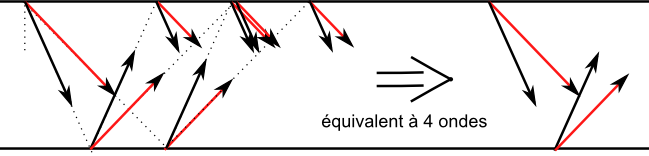
\includegraphics[scale=0.5]{./images/lamb_expli.png}
\caption{\label{fig1} Schéma de la propagation des ondes dans une plaque \emph{in vacuo}.}
\end{figure}

Il y a donc 4 inconnus au problème (correspondant au 4 amplitudes des ondes). Après application des conditions limites (contraintes normales et tangentielles nulles au interfaces car la plaque est \emph{in vacuo}, on obtient un système de 4 équations à 4 inconnus. Il est ensuite facile d'en tirer l'équation de dispersion des ondes dans le milieu en prenant le determinant de la matrice du système. Celle-ci montre qu'il existe 2 types de modes après recombinaison des ondes T et L: les modes symétriques (notés $S_i$) et anti-symétriques (notés $A_i$) qui correspondent à des ondes de compression et des ondes de flexion. Les champs de déplacements de ses 2 types de modes sont représentés sur le schéma \ref{fig2}.

\begin{figure}[H]
\centering
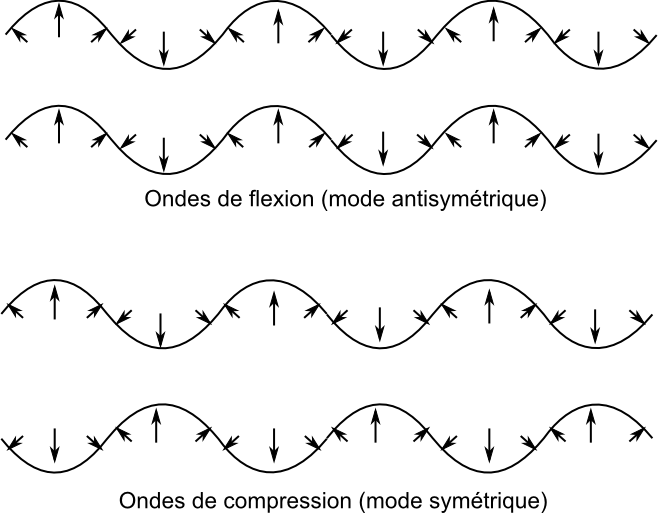
\includegraphics[scale=0.4]{./images/modes.png}
\caption{\label{fig2} Déplacements des 2 modes des ondes de Lamb.}
\end{figure}


\subsection{Courbes de dispersion}

Les courbes de dispersions des ondes de Lamb peuvent être représentées de différentes manières. Dans la figure ~\ref{fig3}, les vitesses de phases sont tracées en fonction de $f.h$ ou $h$ est l'épaisseur de la plaque. 

\begin{figure}[H]
\centering
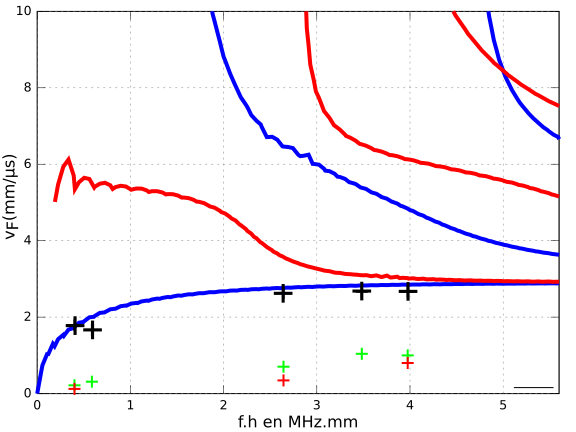
\includegraphics[scale=0.55]{./images/dispercurves_aluminium.png}
\caption{\label{fig3} Courbes de dispersion des ondes de Lamb pour une plaque en aluminium de $5.6mm$ d'épaisseur. En bleu les modes antisymétriques, en rouge les modes symétriques.}
\end{figure}



%------------------------------------------------

\section{Mesure de temps de vols sur une plaque d'acier}
Dans cette section, une onde de Lamb est générée au moyen d'un capteur piézo-électrique dans une plaque d'aluminium de $d = 5.6mm$ d'épaisseur. Le transducteur est placé en incidence normale sur la plaque (avec un couplant), c'est donc les ondes générées par le bord du transducteur qui rayonnent dans la plaque et se combinent pour former les ondes de Lamb. Cette approche à l'avantage de générer tout les modes de Lamb quasiment au même point alors que dans le cas d'une incidence oblique chaque mode a besoin d'une distance différente pour être généré à partir des recombinaisons des ondes T et L.
\bigskip
\emph{Stricto sensu}, se sont des ondes de Lamb généralisées qui sont produites: c'est la généralisation des ondes de Lamb pour une plaque dans un fluide (et pas le vide). Un rayonnement de ces ondes est possible dans le fluide mais extrêmement faible du fait de la rupture d'impédance air-solide. Toutefois, il est nécessaire de faire attention de ne pas laisser du couplant sur la cale servant à garder les 2 transducteurs à une distance fixe car il est alors possible d'avoir une perte de signal liée au rayonnement de l'onde de Lamb dans la cale.
Le but étant de valider les courbes trouvées précédemment, le temps de vol d'impulsions pour différentes fréquences (bursts de 3 cycles) sont relevés avec un deuxième capteur piézo-électrique placé à une distance connue de l'émetteur. Les points représentés figure ~\ref{fig2} sont obtenues à partir des vitesses calculées en fonction des temps de vols (v=d/t).

\bigskip

Le mode A0 est bien identifié, tout les autres points semblent faux. Durant la mesure, nous avons cherché à identifier d'autres paquets d'ondes. Or il semblerait que tout les autres modes doivent apparaître avant l'impulsion que nous avons pris comme référence et non après car leurs vitesses sont plus élevés. Les signaux que nous avons mesurés sont donc probablement des échos du mode A0 et non pas d'autres modes qui eux sont plus atténués.
Le mode A0 est le mode le plus rapide car c'est celui qui se rapproche le plus d'une onde de compression: ce sont les ondes longitudinales les plus rapides.

\bigskip 

Se genre de mesure est très hasardeuse car les différents paquets d'onde se confondent très vite quand on monte en fréquence et se propagent à des vitesses différentes, il est donc difficile de retrouver les courbes de dispersions par cette méthode.


%------------------------------------------------

\section{Utilisation d'un EMAT}
EMAT est une abréviation pour "ElectroMagnetic Acoustic Transducer": ce sont des transducteurs utilisant un gros aimant permanent générant un fort champ magnétique ainsi qu'une bobine générant un champ magnétique fluctuant plus faible pour induire une force de Lorentz dans les pièces métalliques, de cette force découle une onde élastique (cela peut aussi fonctionner par magnétostriction). Le phénomène inverse permet la mesure du champ de contrainte dans le matériau.

\bigskip
L'utilisation des EMAT comporte plusieurs avantages:
\begin{itemize}
\item la génération de l'onde peut se faire sans contact, il n'y a donc pas de couplant nécessaire. De plus, il est facile de contrôler des pièces rugueuses, sales ou aillant un revêtement de faible épaisseur non conducteur (de type gaine isolante),
\item tout les types d'onde peuvent être générés, en particulier les ondes modales tels que les ondes de Lamb ou Rayleigh, ainsi que des ondes TH (transverses horizontales) qui ont l'avantage de ne pas générer d'autres ondes par conversion de modes. 
\end{itemize} 

Cependant se type de transducteur souffre de plusieurs limitations:
\begin{itemize}
\item Du fait de l'excitation magnétique, le matériau à contrôler doit être un conducteur électrique ou posséder un revêtement conducteur,
\item la génération de l'onde se faisant dans la matériau, une zone morte se trouve en surface au niveau de l'émetteur.
\end{itemize}

\subsection{Contrôle d'un tuyau}
Le contrôle d'un tuyau en acier de $8 mm$ d'épaisseur et $17cm$ de diamètre est effectué à l'aide d'un mobile équipé d'un EMAT. Le tout est relié à un boîtier Temate Powerbox. Le tableau \ref{tab1} liste les fréquences permettant la propagation des modes de Lamb dans le tuyau considéré. 

\begin{figure}[H]
\centering
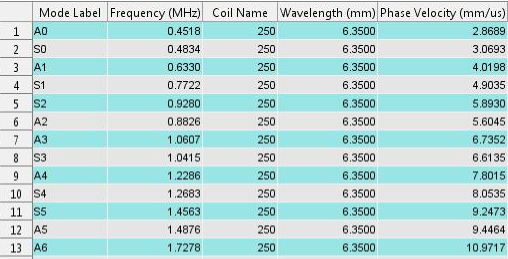
\includegraphics[scale=0.4]{./images/table_dispersion.jpg}
\caption{\label{tab1} Tableau des modes de Lamb pour un tuyau de $8mm$ d'épaisseur en acier.}
\end{figure}

Des coupures et changements d'épaisseurs sont visibles sur le tuyau, se sont ces défauts que l'on cherche à retrouver ici. Une comparaison des signaux avec et sans défaut est présentée figure ~\ref{fig4}. L'excitation est faite à $f = 450 kHz$ afin d'exciter le mode A0. L'onde générée se propage des 2 côtés de l'émetteur: dans le sens horaire et anti-horaire.

\begin{figure}[H]
\centering
\includegraphics[scale=0.06]{./images/comp_lamb.png}
\caption{\label{fig4} A gauche, signal acquit pour un contrôle sur une section du tuyau sans défaut. A droite, un défaut (coupure).}
\end{figure}

Le premier écho de la figure de gauche correspond à la propagation des ondes de Lamb sur le périmètre complet du tuyau. Sur la droite, un écho est visible encore plus tôt: celui-ci correspond à l'onde réfléchie sur le défaut étant revenue au niveau du capteur et aillant donc parcourue une plus faible distance que le périmètre (voir schéma ~\ref{schema1}. 

\begin{figure}[H]
\centering
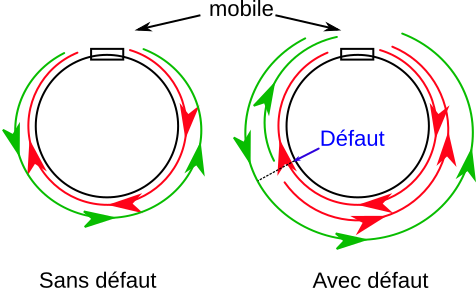
\includegraphics[scale=0.5]{./images/schema_comp_lamb.png}
\caption{\label{schema1} A gauche,schéma pour un contrôle sur une section du tuyau sans défaut. A droite, un défaut (coupure). Les flèches rouges symbolisent le trajet de l'onde dans le sens horaire, les flèches vertes le sens anti-horaire.}
\end{figure}

En mesurant les temps de vol de l'écho du défaut et celui du périmètre complet, il est possible de calculer à quel distance se trouve le défaut du mobile. Il suffit alors de légèrement décaler le mobile pour savoir de quel côté se trouve le défaut et donc le localiser précisément. A l'inverse des méthodes comme le TOFD, la seul indication sur la géométrie du défaut qui peut être obtenue est sa longueur. Par cette méthode, tout les défauts de type coupures sont bien visible, les légers changements d'épaisseurs restent cependant invisibles. En utilisant un autre mode de Lamb (S0), ils deviennent détectables.
\bigskip
Il y a cependant des configurations pour lesquelles les défauts sont indétectables: s'ils se trouvent sous le capteur ou bien à l'opposé du tuyau, les temps de vol ne seront pas modifiés car les échos liés au défauts seront confondus avec ceux de l'onde de référence. Il est donc nécessaire d'effectuer 2 mesures avec le mobile se trouvant à des endroits différents sur le périmètre du tuyau pour affirmer que celui-ci est sain.



\section{Conclusion}
L'utilisation des ondes de Lamb pour le contrôle non destructif possède plusieurs avantages: les ondes étant guidées, il est possible de contrôler des pièces complexes en suivant leurs profils et ce, sur des distance assez grande (l'atténuation est faible). De plus, des transducteurs magnétiques (EMAT) permettent une génération facile du mode de Lamb voulu. Se genre de dispositif est particulièrement adapté au contrôle de tuyauterie, car les ondes générées se propagent loin et sont sensibles au variations de diamètres qui peuvent être induits par la corrosion ainsi qu'a tout défaut intérieur ou extérieur de type coupure. Il est également possible de contrôler des pièces sans enlever les gaines isolantes ou anti-corrosives,ou même des pipelines sans les déterrer.

%----------------------------------------------------------------------------------------
%	REFERENCE LIST
%----------------------------------------------------------------------------------------

\begin{thebibliography}{99} % Bibliography - this is intentionally simple in this template

\bibitem[Lamb]{Lamb}
Lamb, H. 1917.
\newblock"On Waves in an Elastic Plate.
\newblock {\em Proc. Roy. Soc. London, Ser. A 93, 114–128}
 
\end{thebibliography}

%----------------------------------------------------------------------------------------

\end{multicols}

\end{document}
